\documentclass[UTF8]{article}
\usepackage{graphicx}
\usepackage{subfigure}
\usepackage{amsmath}
\usepackage{makecell}
\usepackage[utf8]{inputenc}
\usepackage[space]{ctex} %中文包
\usepackage{listings} %放代码
\usepackage{xcolor} %代码着色宏包
\usepackage{CJK} %显示中文宏包
\usepackage{float}
\usepackage{diagbox}
\usepackage{bm}
\usepackage{ulem} 
\usepackage{amssymb}
\usepackage{soul}
\usepackage{color}
\usepackage{geometry}
\usepackage{fancybox} %花里胡哨的盒子
\usepackage{xhfill} %填充包, 可画分割线 https://www.latexstudio.net/archives/8245
\usepackage{multicol} %多栏包
\usepackage{enumerate} %可以方便地自定义枚举标题
\usepackage{multirow} %表格中多行单元格合并
\usepackage{wasysym} %可以使用wasysym里的一堆奇奇怪怪的符号
\usepackage{hyperref} % url
%%%%%%%%%%%%%%%伪代码%%%%%%%%%%%%%%%
\usepackage{amsmath}
\usepackage{algorithm}
\usepackage{algorithmicx}
\usepackage[noend]{algpseudocode}
%%%%%%%%%%%%%%%画图包%%%%%%%%%%%%%%%
\usepackage{tikz}
\usepackage{pgfplots} % http://pgfplots.sourceforge.net/gallery.html
\usetikzlibrary{pgfplots.patchplots} % 拟合支持
\usetikzlibrary{arrows,shapes,automata,petri,positioning,calc} % 状态图支持
\usetikzlibrary{arrows.meta} % 箭头
\usetikzlibrary{shadows} % 阴影支持
\usepackage{forest} % 画树

\geometry{left = 1.5cm, right = 1.5cm, top=1.5cm, bottom=2cm}

\definecolor{mygreen}{rgb}{0,0.6,0}
\definecolor{mygray}{rgb}{0.5,0.5,0.5}
\definecolor{mymauve}{rgb}{0.58,0,0.82}
\lstset{
	backgroundcolor=\color{white}, 
	%\tiny < \scriptsize < \footnotesize < \small < \normalsize < \large < \Large < \LARGE < \huge < \Huge
	basicstyle = \footnotesize,       
	breakatwhitespace = false,        
	breaklines = true,                 
	captionpos = b,                    
	commentstyle = \color{mygreen}\bfseries,
	extendedchars = false,
	frame = shadowbox, 
	framerule=0.5pt,
	keepspaces=true,
	keywordstyle=\color{blue}\bfseries, % keyword style
	language = C++,                     % the language of code
	otherkeywords={string}, 
	numbers=left, 
	numbersep=5pt,
	numberstyle=\tiny\color{mygray},
	rulecolor=\color{black},         
	showspaces=false,  
	showstringspaces=false, 
	showtabs=false,    
	stepnumber=1,         
	stringstyle=\color{mymauve},        % string literal style
	tabsize=4,          
	title=\lstname           
}

%\sum\nolimits_{j=1}^{M}   上下标位于求和符号的水平右端,
%\sum\limits_{j=1}^{M}   上下标位于求和符号的上下处,
%\sum_{j=1}^{M}  对上下标位置没有设定,会随公式所处环境自动调整。

%%%%%%%%%%%%%画图包%%%%%%%%%%%%%
\usepackage{tikz}
%%%%%%%%%%%%%好看的矩形%%%%%%%%%%%%%
\tikzset{
  rect1/.style = {
    shape = rectangle,% 指定样式
    minimum height=2cm,% 最小高度
    minimum width=4cm,% 最小宽度
    align = center,% 文字居中
    drop shadow,% 阴影
  }
}
%%%%%%%%%%%%%画图背景包%%%%%%%%%%%%%
\usetikzlibrary{backgrounds}

%%%%%%%%%%%%%在tikz中画一个顶点%%%%%%%%%%%%%
%%%%%%%%%%%%%#1:node名称%%%%%%%%%%%%%
%%%%%%%%%%%%%#2:位置%%%%%%%%%%%%%
%%%%%%%%%%%%%#3:标签%%%%%%%%%%%%%
\newcommand{\newVertex}[3]{\node[circle, draw=black, line width=1pt, scale=0.8] (#1) at #2{#3}}
%%%%%%%%%%%%%在tikz中画一条边%%%%%%%%%%%%%
\newcommand{\newEdge}[2]{\draw [black,very thick](#1)--(#2)}
%%%%%%%%%%%%%在tikz中放一个标签%%%%%%%%%%%%%
%%%%%%%%%%%%%#1:名称%%%%%%%%%%%%%
%%%%%%%%%%%%%#2:位置%%%%%%%%%%%%%
%%%%%%%%%%%%%#3:标签内容%%%%%%%%%%%%%
\newcommand{\newLabel}[3]{\node[line width=1pt] (#1) at #2{#3}}

%%%%%%%%%%%%%强制跳过一行%%%%%%%%%%%%%
\newcommand{\jumpLine} {\hspace*{\fill} \par}
%%%%%%%%%%%%%关键点指令,可用itemise替代%%%%%%%%%%%%%
\newcommand{\keypoint}[2]{$\bullet$\textbf{#1}\quad#2\par}
%%%%%%%%%%%%%<T>平均值表示%%%%%%%%%%%%%
\newcommand{\average}[1]{\left\langle #1\right\rangle }
%%%%%%%%%%%%%表格内嵌套表格%%%%%%%%%%%%%
\newcommand{\tabincell}[2]{\begin{tabular}{@{}#1@{}}#2\end{tabular}}
%%%%%%%%%%%%%大黑点item头%%%%%%%%%%%%%
\newcommand{\itemblt}{\item[$\bullet$]}
%%%%%%%%%%%%%大圈item头%%%%%%%%%%%%%
\newcommand{\itemc}{\item[$\circ$]}
%%%%%%%%%%%%%大星星item头%%%%%%%%%%%%%
\newcommand{\itembs}{\item[$\bigstar$]}
%%%%%%%%%%%%%右▷item头%%%%%%%%%%%%%
\newcommand{\itemrhd}{\item[$\rhd$]}
%%%%%%%%%%%%%定义为%%%%%%%%%%%%%
\newcommand{\defas}{=_{df}}
%%%%%%%%%%%%%偏导%%%%%%%%%%%%%
\newcommand{\partialx}[2]{\frac{\partial #1}{\partial #2}}
%%%%%%%%%%%%%蕴含%%%%%%%%%%%%%
\newcommand{\imp}{\rightarrow}
%%%%%%%%%%%%%上取整%%%%%%%%%%%%%
\newcommand{\ceil}[1]{\lceil#1\rceil}
%%%%%%%%%%%%%下取整%%%%%%%%%%%%%
\newcommand{\floor}[1]{\lfloor#1\rfloor}

%%%%%%%%%%%%%双线分割线%%%%%%%%%%%%%
\newcommand*{\doublerule}{\hrule width \hsize height 1pt \kern 0.5mm \hrule width \hsize height 2pt}
%%%%%%%%%%%%%双线中间可加东西的分割线%%%%%%%%%%%%%
\newcommand\doublerulefill{\leavevmode\leaders\vbox{\hrule width .1pt\kern1pt\hrule}\hfill\kern0pt }
%%%%%%%%%%%%%左大括号%%%%%%%%%%%%%
\newcommand{\leftbig}[1]{\left\{\begin{array}{l}#1\end{array}\right.}
%%%%%%%%%%%%%矩阵%%%%%%%%%%%%%
\newcommand{\mat}[2]{\left[\begin{array}{#1}#2\end{array}\right]}
%%%%%%%%%%%%%可换行圆角文本框%%%%%%%%%%%%%
\newcommand{\ovalboxn}[1]{\ovalbox{\tabincell{l}{#1}}}
%%%%%%%%%%%%%设置section的counter, 使从1开始%%%%%%%%%%%%%
\setcounter{section}{0}

%%%%%%%%%%%%%Colors%%%%%%%%%%%%%
\newcommand{\lightercolor}[3]{% Reference Color, Percentage, New Color Name
    \colorlet{#3}{#1!#2!white}
}
\newcommand{\darkercolor}[3]{% Reference Color, Percentage, New Color Name
    \colorlet{#3}{#1!#2!black}
}
\definecolor{aquamarine}{rgb}{0.5, 1.0, 0.83}
\definecolor{Seashell}{RGB}{255, 245, 238} %背景色浅一点的
\definecolor{Firebrick4}{RGB}{255, 0, 0}%文字颜色红一点的
\lightercolor{gray}{20}{lgray}
\newcommand{\hlg}[1]{
	\begingroup
		\sethlcolor{lgray}%背景色
		\textcolor{black}{\hl{\mbox{#1}}}%textcolor里面对应文字颜色
	\endgroup
}


\title{机器学习概论 实验报告 \\ \Large Lab2: SVM}

\begin{document}
\maketitle
\section{理论基础}
\subsection{基本原理}
\begin{itemize}
	\item \textbf{支持向量机}(support vector machine, SVM)是一种二分类模型, 它的基本模型是定义在特征空间上的间隔最大的线性分类器, 间隔最大使它有别于感知机. SVM 还包括核技巧, 这使它成为实质上的非线性分类器. SVM 的学习算法就是求解凸二次规划的最优化算法.
	\item \textbf{基本思想}: 求解能够正确划分数据集并且几何间隔最大的分离超平面.
	\begin{figure}[H]
		\centering
		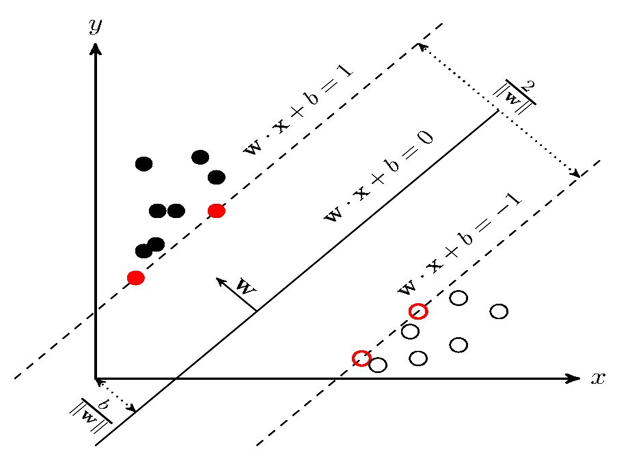
\includegraphics[width=\linewidth/5*2]{SVM.png}
		\caption{SVM 图解}
	\end{figure}
	\item SVM 的类别
	\begin{itemize}
		\item \textbf{线性支持向量机}: 就是上述求解凸二次优化问题的模型
		\item \textbf{近似线性支持向量机}: 当数据集不能严密可分时, 我们可以引入松弛因子, 这样就能保证点被超平面"分开"
		\item \textbf{非线性支持向量机}: 有了核技巧的帮助, 就可以将 SVM 推广到非线性情况.
	\end{itemize}
\end{itemize}
\section{数学基础}
根据数据集的情况, 我决定选用 \textbf{近似线性支持向量机}.
\subsection{优化目标}
\noindent 在利用软间隔的情况下, 最优化目标变为:
$$\min\limits_{\bm{\omega},b}\frac{1}{2}\|\bm{\omega}\|^2+C\sum\limits_{i=1}^ml_{hinge}(y_i(\bm{\omega}^T\bm{x}_i+b)-1)$$
其中 $l_{hinge}$是 \hlg{hinge损失函数}:
$$l_{hinge}(z)=\max(0,1-z)$$
因此最终优化目标可以写为:
$$\min\limits_{\bm{\omega},b}\frac{1}{2}\|\bm{\omega}\|^2+C\sum\limits_{i=1}^m\xi_i$$
$$s.t.\quad\left\{\begin{array}{l}
	y_i(\bm{\omega}\bm{x}_i+b)\ge1-\xi_i\\
	\xi_i\ge0,i=1,2,\cdots,m
\end{array}\right.$$
这里
$$\xi_i=\max(0,1-y_i(\bm{\omega}^T\bm{x}_i+b))$$
\subsection{转化为对偶问题}
\noindent 可以写出拉格朗日函数:
\begin{align*}
	L(\bm{\omega},b,\bm{\alpha},\bm{\xi},\bm{\mu})=&\frac{1}{2}\|\bm{\omega}\|^2+C\sum\limits_{i=1}^m\xi_i\\
	& +\sum\limits_{i=1}^m\alpha_i(1-\xi_i-y_i(\bm{\omega}^T\bm{x}_i+b))-\sum\limits_{i=1}^m\mu_i\xi_i
\end{align*}
这里 $\alpha_i,\mu_i\ge0$.\\
让 $L(\bm{\omega},b,\bm{\alpha},\bm{\xi},\bm{\mu})$ 对$\bm{\omega},b,\xi_i$ 求偏导并带回, 可以得到对偶问题:
$$\max\limits_{\bm{\alpha}}\sum\limits_{i=1}^m\alpha_i-\frac{1}{2}\sum\limits_{i=1}^m\sum\limits_{j=1}^m\alpha_i\alpha_jy_iy_j\bm{x}_i^T\bm{x}_j$$
$$s.t.\quad\left\{\begin{array}{l}
	\sum\limits_{i=1}^m\alpha_iy_i=0\\
	0\le\alpha_i\le C,\ i=1,2,\cdots,m
\end{array}\right.$$
而通过$\alpha_i$能够求出$\omega$:
$$\bm{\omega}=\sum\limits_{i=1}^m\alpha_iy_i\bm{x}_i$$
也能求出$b$:
\begin{align*}
	b=\frac{1}{|S|}\sum\limits_{s\in S}\left(y_s(1-\xi_i) - \sum\limits_{i\in S}\alpha_iy_i\bm{x}_i^T\bm{x}_s\right)
\end{align*}
\subsection{KKT条件条件}
\noindent 其相应 KKT 条件为:
$$\left\{\begin{array}{l}
	\alpha_i\ge0,\qquad\mu_i\ge0\\
	y_if(\bm{x}_i)-1+\xi_i\ge0\\
	\alpha_i(y_if(\bm{x}_i)-1+\xi_i)=0\\
	\xi_i\ge 0,\ \mu_i\xi_i=0
\end{array}\right.$$
根据 KKT 条件我们能够知道, 
\begin{itemize}
	\item 当 $\alpha_i=0$ 时, 该样本对 $f(\bm{x})$ 不会有任何影响,
	\item 当$C>\alpha_i>0$ 时, 必然有 $y_if(\bm{x}_i)=1-\xi_i=1$, 即该样本是支持向量
	\item 当 $\alpha=C$, 则$\mu_i=0$, 此时若$\xi_i\le1$, 则样本落在最大间隔内部; 若$\xi_i>1$ , 则样本被错误分类.
\end{itemize}
\section{更新算法}
\subsection{Gradient Descent 算法(GD)}
\noindent 这个算法的理论基础上一次报告已经介绍过了, 这里再展示一下算法流程:
\begin{algorithm}[H]
	\caption{GD}
	\begin{algorithmic}[1] %每行显示行号
		\Require 训练的 epochs $M$; 初始化 $\beta=(w,b)$, 学习率 $\alpha$
		\For{每个 epoch}
			\For{每个训练样本 $x_i$}
				\State 计算误差 $e=1-y_i(w\cdot x_i+b)$
				\If{$e > 0$}
					\State $w=(1-\eta)w+\eta Cx_iy_i$
					\State $b=b+\eta Cy_i$
				\EndIf
			\EndFor
		\EndFor
	\end{algorithmic}
\end{algorithm}

\subsection{Stochastic Gradient Descent 算法(SGD)}
\noindent 这个算法的理论基础上一次报告已经介绍过了, 这里再展示一下算法流程:
\begin{algorithm}[H]
	\caption{SGD}
	\begin{algorithmic}[1] %每行显示行号
		\Require 训练的 epochs $M$; 初始化 $\beta=(w,b)$, 学习率 $\alpha$
		\For{每个 epoch}
			\For{每个训练样本 $x_i$}
				\State 按这个公式计算所有数据的误差 $e_i=1-y_i(w\cdot x_i+b)$
				\State 取误差最大的一项 $i=\arg\max\limits_ie_i$
				\If{$e_i\le 0$}
					\State break
				\EndIf
				\State $w=(1-\eta)w+\eta Cx_iy_i$
				\State $b=b+\eta Cy_i$
			\EndFor
		\EndFor
	\end{algorithmic}
\end{algorithm}

\subsection{SMO算法}
\subsubsection{选取待优化的两个参数}
\begin{itemize}
	\item 选取$\alpha_i$: 
	\begin{enumerate}[1. ]
		\item 首先选取违反 $0<\alpha_i<C \Rightarrow y_if(\bm{x}_i)=1$ 的点
		\item 其次选择违反 $\alpha_i=0\Rightarrow y_if(\bm{x}_i)\ge1$ 的点和 $\alpha_i=C\Rightarrow y_if(\bm{x}_i)\le1$ 的点.
	\end{enumerate}
	\item 选取$\alpha_j$: 第二个变量的选择应当使得目标函数值减小最快
\end{itemize}
\subsubsection{更新两个参数}
\begin{itemize}
\item 求出 $$\alpha^{newunc}_j=\alpha_j^k+\frac{y_j(E_i-E_j)}{K_{ii}+K_{jj}-2K_{12}}$$
\item 为了保证其界限, 需要如下操作:
$$\alpha_j^{k+1}=\left\{\begin{array}{ll}
	H & \alpha_j^{newunc} > H\\
	\alpha_j^{newunc} & L\le  \alpha_j^{newunc}\le H\\
	L &  \alpha_j^{newunc} < L
\end{array}\right.$$
\item 进而可以求出 $\alpha_i^{k+1}$
\end{itemize}
\subsubsection{更新b}
\begin{itemize}
\item 按如下公式更新b:
$$b^{new}=\frac{b_i^{new}+b_j^{new}}{2}$$
其中$$\begin{array}{l}
b_i^{new}=-E_i-y_iK_{ii}(\alpha_i^{new}-\alpha_i^{old})-y_jK_{ji}(\alpha_j^{new}-\alpha_j^{old})+b^{old}\\
b_j^{new}=-E_j-y_iK_{ij}(\alpha_i^{new}-\alpha_i^{old})-y_jK_{jj}(\alpha_j^{new}-\alpha_j^{old})+b^{old}
\end{array}$$
\end{itemize}


\section{实验结果}
\subsection{总体对比}
\begin{center}
\begin{tabular}{|c|c|c|c|c|}
\hline
模型/算法 & 数据集 & 训练集准确度 & 测试集准确度 & 迭代次数\\
\hline
GD & s-svm & 0.9571 & 0.9714 & 30 \\
SGD & s-svm & 0.9285 & 0.9714 & 100000 \\
SMO & svm & 0.7571 & 0.8642 & 200 \\
sklearn(与SMO相同条件) & svm & 0.7142 & 0.6667 & - \\
\hline
\end{tabular}
\end{center}
\noindent 可以看到就第一个简单的数据集(s-svm)而言, \hlg{GD 算法} 和 \hlg{SGD 算法}都能够达到非常好的表现. 而对于比较奇怪的数据集(svm)来说, GD/SGD算法表现不佳(未展示), 而 \hlg{SMO 算法} 则表现得好一些, 甚至好于同等条件下的 sklearn(但未进行较好调参).
\subsection{GD 算法实验结果}
\begin{itemize}
	\item 经过调整参数, 可以得到在\textbf{学习率为 0.01, epoch为30时}, 能够在\textbf{训练集上达到 0.9571 的准确率}, 在\textbf{测试集上达到 0.9714 的准确率}.
	\item 训练结果可视化:
	\begin{figure}[H]
		\begin{minipage}[H]{0.5\linewidth}
			\centering
			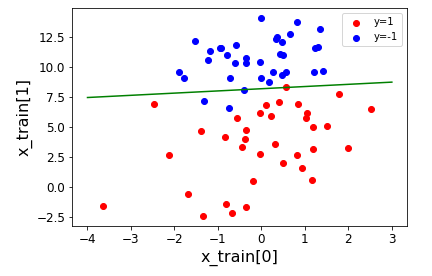
\includegraphics[width=\linewidth]{gd_train.png}
			\caption{GD算法在训练集上的表现}
		\end{minipage}
		\begin{minipage}[H]{0.5\linewidth}
			\centering
			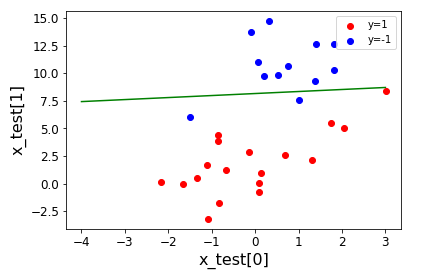
\includegraphics[width=\linewidth]{gd_test.png}
			\caption{GD算法在测试集上的表现}
		\end{minipage}
	\end{figure}
\end{itemize}
\subsection{SGD 算法实验结果}
\begin{itemize}
	\item 经过调整参数, 可以得到在\textbf{学习率为 0.001, epoch为 100000 时}, 能够在\textbf{训练集上达到 0.9285 的准确率}, 在\textbf{测试集上达到 0.9714 的准确率}.
	\item 训练结果可视化:
	\begin{figure}[H]
		\begin{minipage}[H]{0.5\linewidth}
			\centering
			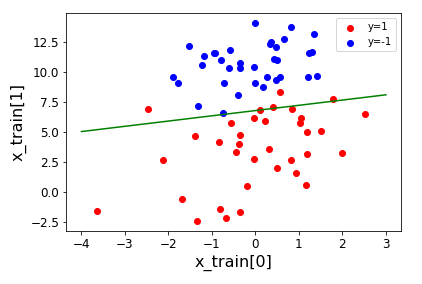
\includegraphics[width=\linewidth]{sgd_train.png}
			\caption{SGD算法在训练集上的表现}
		\end{minipage}
		\begin{minipage}[H]{0.5\linewidth}
			\centering
			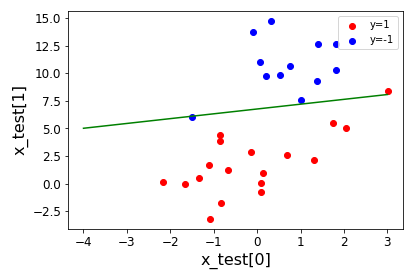
\includegraphics[width=\linewidth]{sgd_test.png}
			\caption{SGD算法在测试集上的表现}
		\end{minipage}
	\end{figure}
\end{itemize}
\subsection{SMO 算法实验结果}
\begin{itemize}
	\item 经过调整参数, 可以得到在\textbf{epoch为 200 时}, 能够在\textbf{训练集上达到 0.7571 的准确率}, 在\textbf{测试集上达到 0.8642 的准确率}.
	\item 训练结果可视化:
	\begin{figure}[H]
		\begin{minipage}[H]{0.5\linewidth}
			\centering
			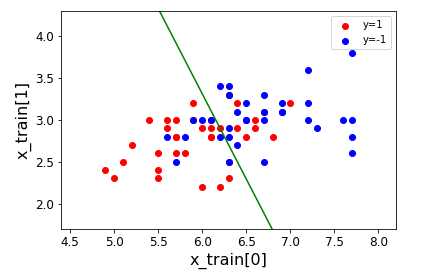
\includegraphics[width=\linewidth]{smo_train.png}
			\caption{SMO 算法在训练集上的表现}
		\end{minipage}
		\begin{minipage}[H]{0.5\linewidth}
			\centering
			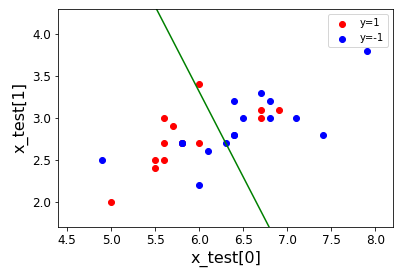
\includegraphics[width=\linewidth]{smo_test.png}
			\caption{SMO 算法在测试集上的表现}
		\end{minipage}
	\end{figure}
\end{itemize}

\section{实验总结}
\noindent 本次实验和上次实验中均发现对于数据集小的情况下, \hlg{GD 算法} 往往能够优于 \hlg{SGD 算法}(些微). 而本次实验中的 \hlg{SMO 算法} 对于小数据集也颇有杀鸡而用牛刀之意. 因此, 针对数据集不同, 我们应该选择合适的方法.


\end{document}





